\documentclass[12pt,a4paper]{article}
\usepackage[latin2]{inputenc}
\usepackage{graphicx}
\usepackage{ulem}
\usepackage{amsmath}
\usepackage[margin=0.5in]{geometry}
\usepackage[T1]{fontenc}
\usepackage[ampersand]{easylist}
\usepackage[english]{babel}
\usepackage{scrextend}
\usepackage{subfig}
\usepackage{float}
\usepackage{stackengine}
\usepackage{listings}
%\usepackage[demo]{graphicx}
%\usepackage{caption}
%\usepackage{subcaption}
%\usepackage[utf8]{inputenc}
\begin{document}

%%%%%%%%%%%%%%%%%%%%%%%%%%%%%%%%%%%%%%%%%%%%%%%%%%%%%%%%%%%%%%%%%%%%%%%%%%%%%%%%
% Document Setup

\pagenumbering{arabic}
\setcounter{page}{0}

%%%%%%%%%%%%%%%%%%%%%%%%%%%%%%%%%%%%%%%%%%%%%%%%%%%%%%%%%%%%%%%%%%%%%%%%%%%%%%%%
% Title block - Page 0

% Cover page. Clearly indicate the names of the team members.
% Also provide a table comparing the given specs and achieved spec (remember
% this is for the NON-BONUS part of the project only). You also need to provide
% us a percentage-wise break down of area consumed by different sections of
% bias circuit (VNMOS-bias, VPMOS-bias & bias generator circuit) as compared to
% your core circuit area (refer to Figure 3). For area calculation, use
% AMOS = W * L. Also include the area of resistors in your design. Assume that
% the sheet resistance is 5.5 kohm/sq and the minimum length of resistor is
% 1 um

\author{
  Kankanala, Usha\\
  \texttt{ukankana@stanford.edu}\\
  \texttt{SUID:06091239}
  \and
  Lenius, Samuel\\
  \texttt{lenius@stanford.com}\\
  \texttt{SUID:06091240}
}

\title{2015 EE214A Design Project}

\maketitle

%%%%%%%%%%%%%%%%%%%%%%%%%%%%%%%%%%%%%%%%%%%%%%%%%%%%%%%%%%%%%%%%%%%%%%%%%%%%%%%%
% Performance Summary Block - Page 0

\begin{table}[h]
	\centering
	\begin{tabular}{ | l | l | l |}
		\hline
		\textbf{Specfications} & Given Spec & Achieved Spec\\
		\hline
			Gain & 30k$\Omega$  &  34.7k$\Omega$ \\
		\hline
			Bandwidth & 90MHz  &  93MHz \\
		\hline
			Power & 2.0mW  &  1.0mW \\
		\hline
			FOM & 1350  &  3043 \\
		\hline
	\end{tabular}
\end{table}


\begin{table}[h]
	\centering
	\begin{tabular}{ | l | l | l |}
		\hline
		\textbf{Area Breakdown} & $\%$ Core Area & Area (um)\\
		\hline
			Core Area & 100\% & 112$\mu$m\textsuperscript{2}  \\
		\hline
			VNMOS-bias & 19.6\% & 22$\mu$m\textsuperscript{2} \\
		\hline
			VPMOS-bias  & 10.7\%  & 12$\mu$m\textsuperscript{2} \\
		\hline
			Bias Generator & 73.1\% &  82$\mu$m\textsuperscript{2} \\
		\hline
	\end{tabular}
\end{table}

\pagebreak

%%%%%%%%%%%%%%%%%%%%%%%%%%%%%%%%%%%%%%%%%%%%%%%%%%%%%%%%%%%%%%%%%%%%%%%%%%%%%%%%
% Design Outline - Page 1

% Outline of your design. How did you approach this problem? What are some of
% your key design choices? Flow charts and graphs of how the trade-offs are
% connected provide the best clarity in explaining (we'll show some examples in
% class). Half of the grading (i.e. 25 Points) is related to Design Flow,
% Insight and Optimization Strategy. The clarity of your discussion and the
% insight you give, starting on Page 1, is a major factor in doing well for
% these 25 Points.

\section{Design Outline}
\par
Our approach to this design was to first develop sizing ratios of the transistors and their DC relationships to Vx, Vy, Vz and Vo.
We developed the equations necessary to `program' those voltages and to develop what their reasonable ranges are.
Here are some graphs that show the relationships between the output common mode voltage and Vz, and then Vz to Vy given our sizing decisions.
We developed a MATLAB program to quickly estimate critical parameters for a given design, to allow easy investigation of parametric variation.\par

\begin{figure}[H]
	\footnotesize
	\stackunder[5pt]{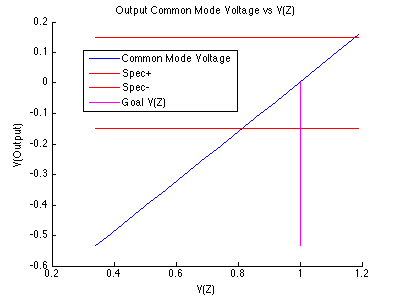
\includegraphics[width=0.5\textwidth]{cmv_vs_vz.png}}{}
	\hfill
	\stackunder[5pt]{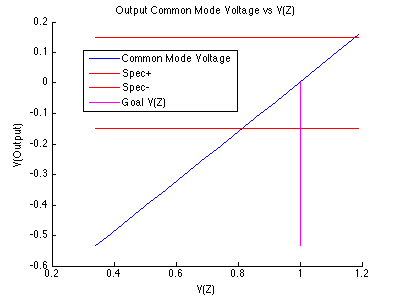
\includegraphics[width=0.5\textwidth]{cmv_vs_vz.png}}{}
\end{figure}


These graphs give rise to a process to choose exactly the value of those voltages based on the size of the transistors.
Here, given the common mode output spec, choosing a size for MN10, and estimating the MN10 backgate gives the needed value of Vz.
Given a size ratio for MN7 to MP8 gives the needed value of Vy, knowing Vz.
Given the size ratio for MP4 to MN6 and knowing the value of Vy gives the gives the necessary ratio of R3 to R4 to program the value of Vy.

{\centering
	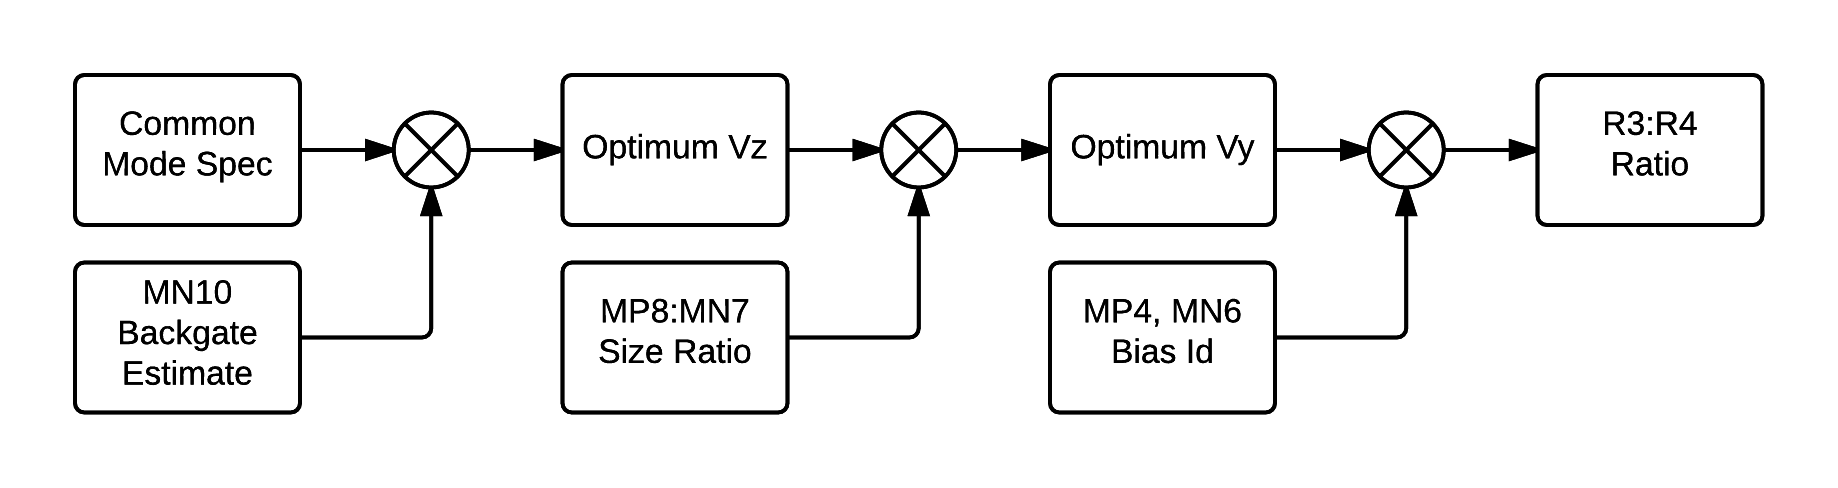
\includegraphics[width=0.7\textwidth]{flowchart_common_mode.png}\par
}

Similarly for Vx, given a goal for MP4 gm (from our chosen distribution of stage gain) we can solve for the ratio of R1 to R2 to program the value of Vx.
Since we have set the K value of MN1 and MP3 equal, the voltage at Vx is selected purely by the ratio of R1 and R2.

{\centering
	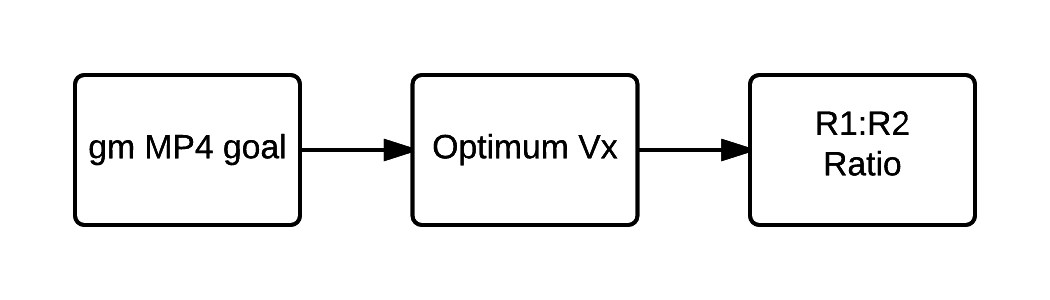
\includegraphics[width=0.4\textwidth]{flowchart_r1_r2.png}\par
}

Once the math was developed to decouple the selection of stage gain to the DC biasing selection, the focus was on gain/speed. 
First we distributed the desired gain for each stage, then choose the vov level to drive the transistors based on the gm/Id plots, 
and then sized the transistors to minimize tau for adjacent stages.\par

The gain budget was based on the X stage having the most gain, since it's easy to get there, getting the balance of gain from the Y stage and then setting the Z stage to cancel out the gain loss of the output CD stage. 
Thus total gain simplifies to X * Y = 30k. \par

By making plots of the sum of tau for adjacent stages vs critical transistor sizing we were able to minimize total tau for the design, with the given gain budget.\par


\pagebreak

%%%%%%%%%%%%%%%%%%%%%%%%%%%%%%%%%%%%%%%%%%%%%%%%%%%%%%%%%%%%%%%%%%%%%%%%%%%%%%%%
% Design Schematic - Page 2

% Schematic diagram of your final design, with component values (i.e. W, L
% values etc.), node voltages and bias currents (from SPICE .op simulation)
% clearly labeled (Spend time to make this schematic complete, readable, and
% clear!). Show component values right next to the components, and currents next
% to the branches (i.e., absolutely, positively do not make us refer to a
% look-up table!). Annotate all transistors with their drain current, gate
% overdrive VOV (from SPICE .op simulation) and W/L.

\section{Design Schematic}

{\centering
	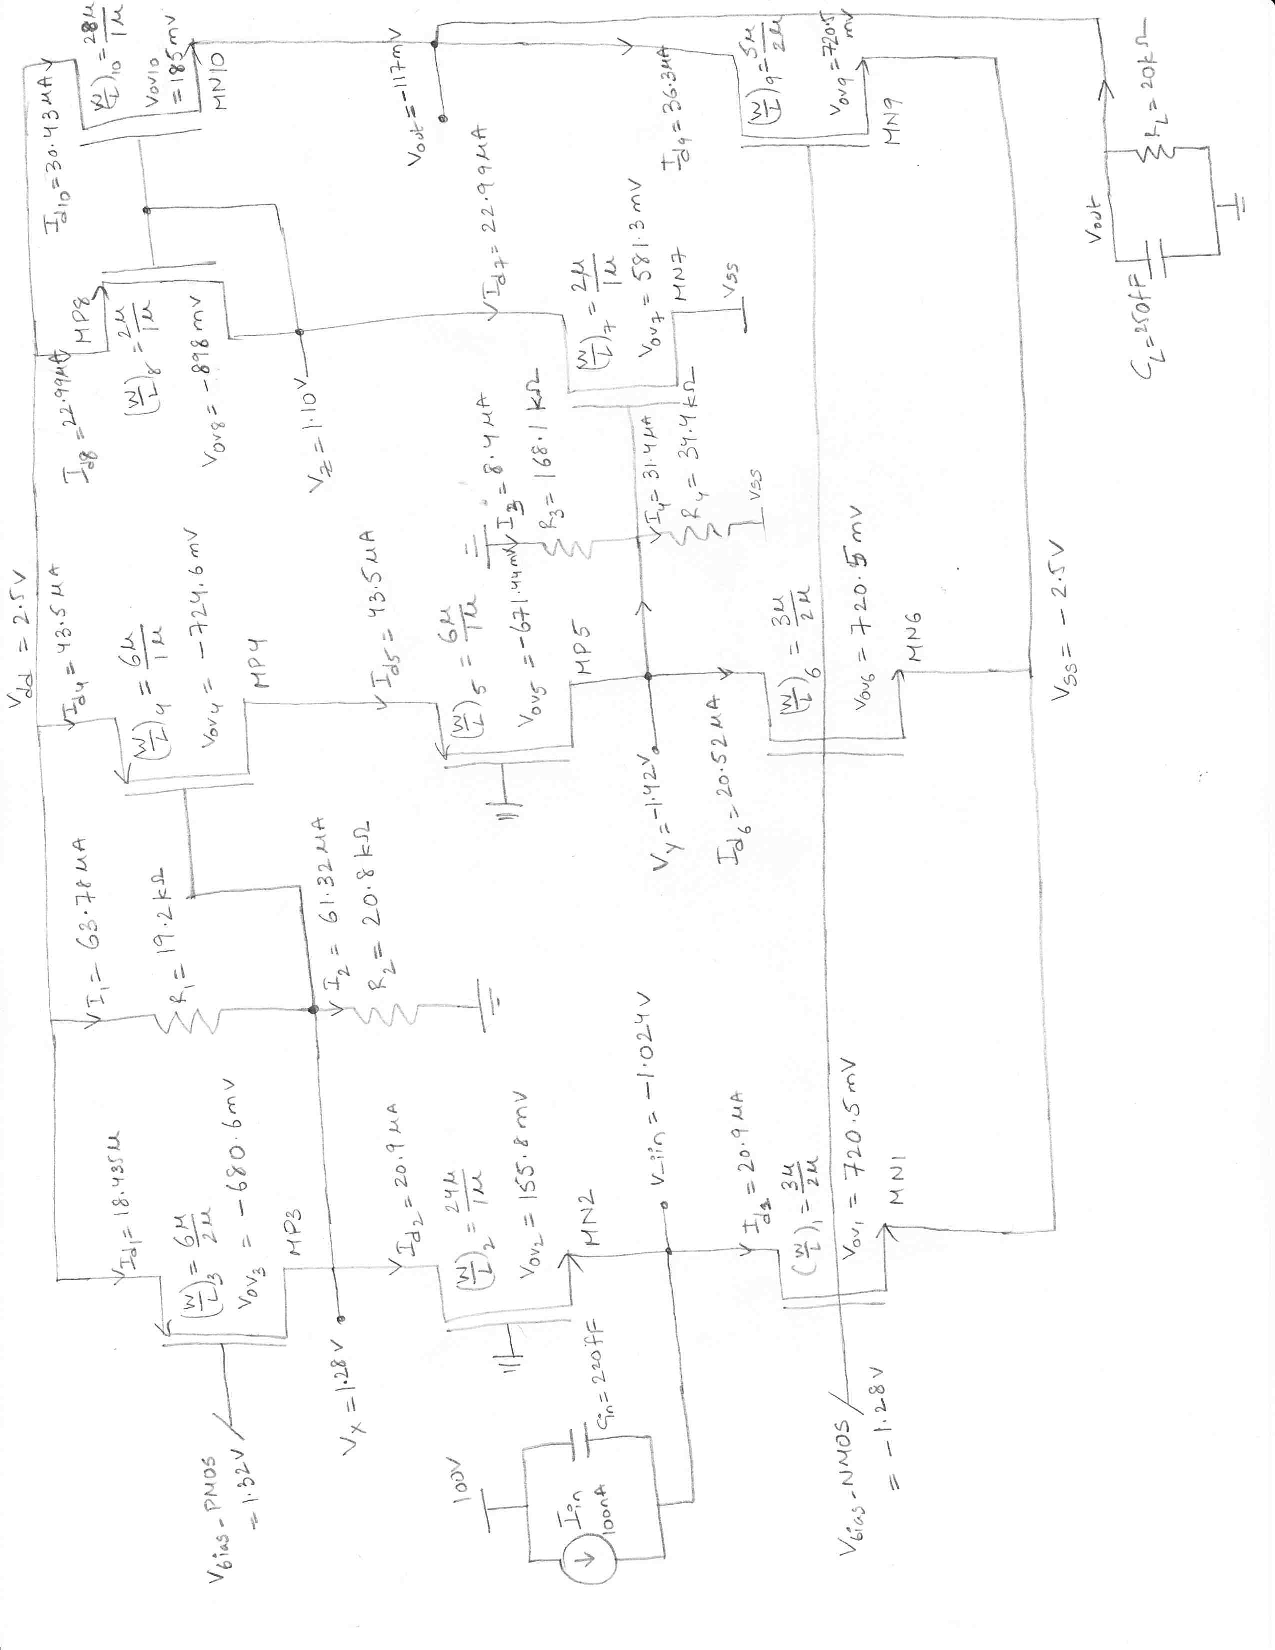
\includegraphics[page=1, angle=270, width=0.9\textwidth]{project_schematic.pdf}\par
}

{\centering
	\includegraphics[page=2, angle=270, width=0.9\textwidth]{project_schematic.pdf}\par
}

\pagebreak

%%%%%%%%%%%%%%%%%%%%%%%%%%%%%%%%%%%%%%%%%%%%%%%%%%%%%%%%%%%%%%%%%%%%%%%%%%%%%%%%
% Calculation of Key Design Parameters - Page 3-6

% Calculation of key design parameters, such as transconductances, bias
% currents, etc. This is the most important section of your report for giving
% critical discussion! Compare the most relevant hand calculated values with
% final SPICE values in a table and discuss discrepancies (percentage
% differences will be clear, you need to show you understand them). Make sure to
% include the total power dissipation of your design (calculated value and SPICE
% result). The lowest power designs will not automatically score the highest
% grades. The methodology you used to justify your design choices and component
% values is far more important (see section on point distribution below).

\section{Calculation of Key Design Parameters}

\textbf{Choice of L}

\begin{itemize}
\item All devices used in current source have a minimum length of 2$\mu$m.
\item All other devices in the amplifier have minimum length of 1$\mu$m. 
Minimum length is used as f$_{t }$ is inversely proportional to L.
\item All devices in bias generator circuit have length $>$=2$\mu$m.
\end{itemize}


\textbf{Bias Generator circuit}

\begin{itemize}
\item Constant gm reference based design is used as bias circuit to 
reduce mismatch errors.
\item Transconductance of bias device (mn300) depends only on R2 and m ( 
m is the ratio of MN300/MN400). Therefore gm can be set precisely.
\item Start-up circuit is used to force the circuit to the desired 
operating point.
\end{itemize}


\textbf{Approximations for hand calculations}

For simpler hand calculations, following approximations are used.

\newcounter{numberedCntBB}
\begin{enumerate}
\item $Cdb=Csb=0.35 Cgs$
\item $Cgs=(\frac{2}{3})WLCox+Cov'W$
\item $Cgd=Cov'W$
\item $gmb=0.2gm$
\setcounter{numberedCntBB}{\theenumi}
\end{enumerate}


\textbf{Stage4}

\begin{itemize}
	\item As per the spec, common mode output voltage (vout) has to be within -0.15v to 0.15v. Since the body is connected to vss, MN10 experiences back gate effect and the threshold voltage is given by:
	\begin{equation}
	\begin{split}
		Vt=Vt_0+ \gamma(\sqrt{2\phi f+V_{sb}}- \sqrt{2}\phi f\\
		Vt_0=0.5V , \gamma=0.6 , 2\phi f=0.8
	\end{split}
	\end{equation}


	\item Stage 4 is a source follower which has a gain given by
	\begin{equation}
		A4=\frac{gm_{10}}{gm_{10}+gmb_{10}+(\frac{1}{R_L})}
	\end{equation}
	\item Gain of stage4 (A4) $<$1 due to back gate effect and the output load. 
	\item To achieve gain closer to 1 (0.6 - 0.7), it is important to size and bias MN10 such that ($gm_{10}+ gmb_{10}) >> (1/R_L)$. 
	\item Transconductance of and drain current of $MN_{10}$ is given by 
	\begin{equation}
		gm_{10}= \mu nCox(\frac{W}{L})vov_{10}
	\end{equation}
	\begin{equation}
		Id_{10}=0.5\mu nCox(\frac{W_{10}}{L_{10}})vov_{10}^2 (1+\lambda (Vdd-Vout))
	\end{equation}
	\item $MN_9$ (bias device for source follower) is sized such that $Id_{10}+ I_{R_L}= Id_9$ and the common mode output voltage does not fall out of range. This device is chosen to be of smaller size to reduce loading on Vout node. 
	\begin{equation}
		\tau_{OUTPUT} = (R_L || \frac{1}{1.2gm_{10}})(C_L+Csb_{10}+Cgd_9+Cdb_9)
	\end{equation}
	\item Cgs10 is assumed to be very small due to boot-strapping.
\end{itemize}


\textbf{Stage 3}

\begin{itemize}
	\item Loading at node Vy increases with the increase in gain of stage 3 due to the miller effect. Hence gain of stage3 is kept low and is fixed at sqrt(2) to compensate for the gain lost in stage 4. Gain of stage3 (CS amplifier with diode connected load):
	\begin{equation}
		|A3|=\frac{gm7}{gm8}=\frac{Vov8}{Vov7}=\frac{Vdd-Vz-abs(Vtp)}{Vy-Vss-Vtn}=\sqrt{2}
	\end{equation}

	\item Choice of Vz from above (stage4) determines Vy.	
	\item Minimum device sizes (W=2$\mu$m, L=1$\mu$m) are used for both MN7 and MP8 to reduce loading on Vy and Vz.
	\begin{equation}
		Id_7=Id_8=0.5\mu nCox(\frac{W_7}{L_7})vov_7^{2} (1+\lambda(Vz-Vss))
	\end{equation}
	\begin{equation}
		\tau_Z=(\frac{1}{gm_8})(Cgs_8+Cdb_8+Cgd_{10}+Cgd_7(1+\frac{1}{|A3|})+Cdb_7)
	\end{equation}
\end{itemize}


\textbf{Stage 2}

\begin{itemize}
	\item Vy from stage Z above determines the required ratio of R3 and R4.
	\begin{equation}
		(\frac{R4}{R3})=\frac{Vss}{Vy}-1
	\end{equation}

	\item Gain of stage Y (Cascode amplifier) is set to 3.
	\begin{equation}
		|A2|=gm4(R3 || R4)
	\end{equation}
	\item $Vov_4$ and $W_{4}$ are optimized to reduce $\tau_X$.
\end{itemize}


\begin{figure}[H]
\centering
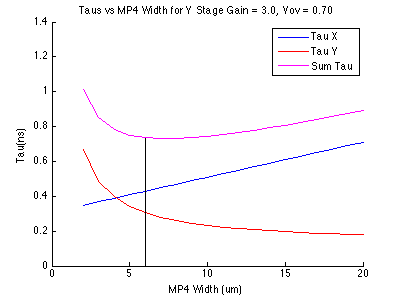
\includegraphics[width=10.63cm,height=7.99cm]{tau_x_y_vs_mp4.png}
\end{figure}


\begin{itemize}
	\item MN6 is sized such that current through MN6 is same as the current through MP4 and MP5. 
	\begin{equation}
		Id4=Id5=Id6=0.5\mu pCox(\frac{W4}{L4})(Vdd-Vx-abs(Vtp))^{2} (1+\lambda (Vdd-Vw)
	\end{equation}
	\item Current through R3 and R4
	\begin{equation}
		I_{R3}+I_{R4}=Vss/(R3+R4)
	\end{equation}
	\begin{equation}
		\tau_Y=(R3 || R4)(Cgs_7+Cgd_7 (1+|A3|)+Cgd_6+Cdb_6+Cgd_5+Cdb_5)
	\end{equation}
\end{itemize}


\textbf{Stage 1}

\begin{itemize}
	\item $Vov_4$ from stage 2 sets $V_X$ which in turn sets the ratio of R1 and R2.
	\begin{equation}
		Vov_4=Vdd-Vx-|Vtp|
	\end{equation}
	\begin{equation}
		(\frac{R1}{R2})=\frac{Vdd}{Vx}-1
	\end{equation}
	\item Gain of stage 1 (Common gate amplifier) is set to 10000.
	\begin{equation}
		|A1|=(R1 || R2)
	\end{equation}
	\item MN1 and MP3 are sized such that Id1 = Id3.
	\item MN2 is sized to reduce $\tau_{IIN}$ node.  $\tau_{IIN}$ is inversely proportional to $gm_2$.
	\begin{equation}
		\tau_{IIN}=(\frac{1}{gm2})(Cin+Cgd_1+Cdb_1+Cgs_2+Csb_2)
	\end{equation}
	\begin{equation}
		\tau_{X}=(R1 || R2)(Cgd_2+Cdb_2+Cgd_3+Cdb_3+Cgs_4+Cgd_4)
	\end{equation}
\end{itemize}



\begin{figure}[h]
\centering
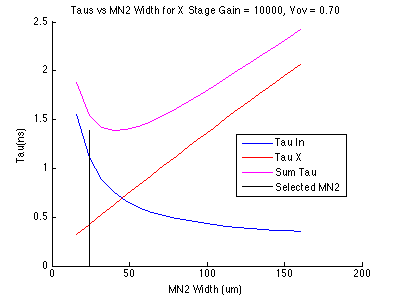
\includegraphics[width=10.63cm,height=7.99cm]{tau_i_x_vs_mn2.png}
\end{figure}


\begin{itemize}
	\item Current through MN1, MN2 and MP3
	\begin{equation}
		Id_{1,2,3}=0.5\mu pCox(\frac{W_3}{L_3})(Vdd-VbiasP-|Vtp|)^{2} (1+\lambda (Vdd-Vx))
	\end{equation}
	\item Current through R1 and R2
	\begin{equation}
		I_{R1}+I_{R2}=Vdd/(R1+R2)
	\end{equation}
\end{itemize}

\textbf{Vovn, Vovp}

\begin{itemize}
	\item Vovn and Vovp are chosen to achieve a reasonable balance between gain, Tau total and Power, and our choice was educated by the gm/Id technology plots.
\end{itemize}
	
\textbf{Total Design Performance}
\begin{equation}
	|A_{TOTAL}|=A1* A2* A3* A4
\end{equation}
\begin{equation}
	\tau_{TOTAL}=\tau_{IIN}+\tau_X+\tau_Y+\tau_Z+\tau_{OUTPUT}
\end{equation}
\begin{equation}
	Power=(Vdd-Vss)(Id_1+Id_4+Id_7+Id_{10})+(\frac{Vdd^{2}}{R1+R2})+(\frac{Vss^{2}}{R3+R4})
\end{equation}

\begin{table}[h]
\centering
\begin{tabular}{|l|l|l|l|l|}
\hline
\textbf{Bias Generator} & Hand calc & Spice & \%Error & Reason for error \\
\hline
$V_{BiasN}$ & -1.300V &  -1.279V &  -1.6\% &  Startup circuit bias \\
\hline
$V_{BiasP}$ & 1.300V &  1.319V & 1.5\%  &  Startup circuit bias \\
\hline
  &   &   &   &   \\
\hline
\textbf{Stage1} & Hand calc & Spice & \%Error & Reason for error \\
\hline
$Id_1$ & 18.3$\mu$A  &  20.9$\mu$A &  14.2\% &  Bias generator error \\
\hline
Vx & 1.300V  & 1.275V  & -1.9\%  &   \\
\hline
$A_X$ & 10k$\Omega$  & 9.86k$\Omega$  & -1.4\%  & Finite $MN_1$ and $MP_3$ output resistance  \\
\hline
$gm_2$ &  210$\mu$S & 268$\mu$S  & 27.6\%  & Bias generator error  \\
\hline
$\tau_{IN} $ & 1.11ns  &   &   &   \\
\hline
$\tau_X $ & 420ps  &   &   &   \\
\hline
  &   &   &   &   \\
\hline
\textbf{Stage2} & Hand calc & Spice & \%Error & Reason for error \\
\hline
$Id_4$ &  36.75$\mu$A & 43.5$\mu$A & 18.4\%  &   \\
\hline
$V_W$ & 1.496V & 1.450V  & -3.2\%  &   \\
\hline
$V_Y$ & -1.550V  & -1.418V  &  -8.5\% & Imbalance between $MP_4$ and $MN_6$ current \\
\hline
$gm_4$ & 105$\mu$S  &  120$\mu$S & 14.3\%  & Error in $V_Y$ \\
\hline
$A_Y$ & -3.0  & -3.25  & 8.3\%  & Error estimating $gm_4$  \\
\hline
$\tau_Y$ & 306ps  &   &   &   \\
\hline
  &   &   &   &   \\
\hline
\textbf{Stage3} & Hand calc & Spice & \%Error & Reason for error \\
\hline
$Id_7$ & 10.25$\mu$A  & 22.9$\mu$A  & 123\%  & Error in $V_Y$ plus finite output resistance  \\
\hline
$V_Z$ & 1.364 & 1.102V  & -19.2\%  & Error in $V_Y$   \\
\hline
$gm_7$ & 45$\mu$S  & 79$\mu$S  & 75.5\%  &  Error in $Id_7$ \\
\hline
$gm_8$ & 31.2$\mu$S & 51$\mu$S   &  63.5\% &  Error in $Id_7$  \\
\hline
$A_Z$ & 1.414  & 1.440  & 1.8\%  &  The benefit of ratiometric design \\
\hline
$\tau_Z$ & 1.92ns  &   &   &  Error in estimating $gm_{8}$ \\
\hline
  &   &   &   &   \\
\hline
\textbf{Stage4} & Hand calc & Spice & \%Error & Reason for error \\
\hline
$Id_{10}$ & 2.96$\mu$A  &  30.43$\mu$A &  928\% & $MN_{10}$'s large width is a big error amplifier  \\
\hline
$V_{OUT}$ & 0.299 & -0.117V  &  -139\% &   \\
\hline
$Vt_{10}$ & 0.999  & 1.034V  &  3.5\% &   \\
\hline
$gm_{10}$ & 91.1$\mu$S   &  327$\mu$S  & 258\%  &   \\
\hline
$gmb_{10}$ & 13.0$\mu$S  &  55.1$\mu$S  & 323\%  &   \\
\hline
$A_{OUT}$ & 0.71 & 0.75  & 5.6\%  &   \\
\hline
$\tau_{OUT}$ & 1.63ns  &   &   & Error in estimating $gm_{10}$  \\

\hline
Total Power &  578$\mu$W & 1.065mW  & 84\%  & Not accounting for bias gen  \\
\hline
Total Gain & 30.04k$\Omega$  & 34.66k$\Omega$   &  15.5\% & Error in estimating gm  \\
\hline
\end{tabular}
\end{table}

\pagebreak

%%%%%%%%%%%%%%%%%%%%%%%%%%%%%%%%%%%%%%%%%%%%%%%%%%%%%%%%%%%%%%%%%%%%%%%%%%%%%%%%
% Bode Diagrams - Page 7

% Simulated Bode Plots of A(jw), magnitude and phase. Clearly annotate the
% achieved gain and bandwidth. Annotate your hand-calculated values in the same
% plots, noting any specific features of interest (either from the results
% themselves or based on what you've learned in hand calculations or scripting
% the design). Plots must be annotated with meaningful comments/observations.

\section{Simulated Bode Plots}

{\centering
	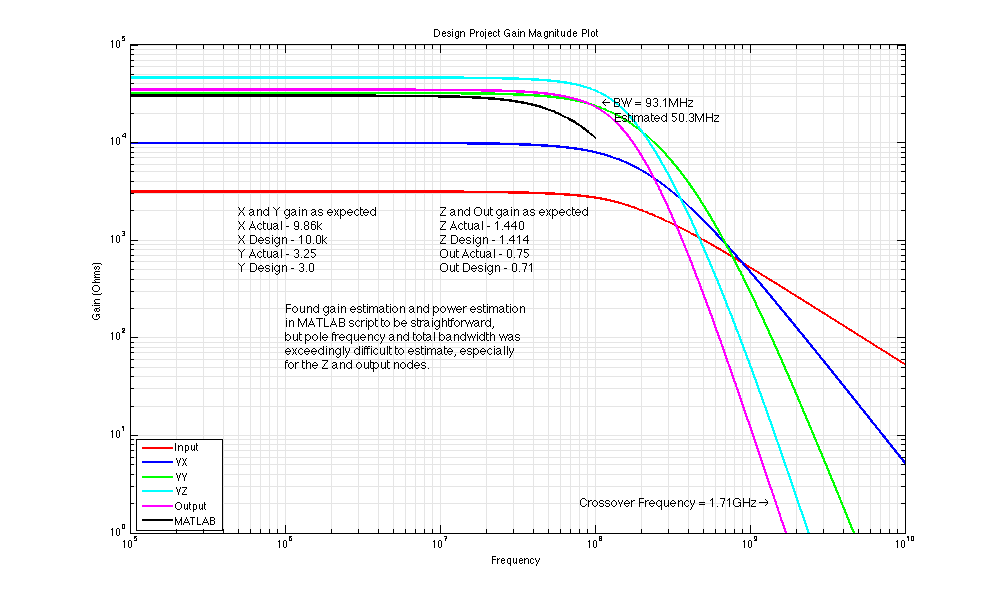
\includegraphics[width=1.1\textwidth]{mag.png}
\par}

{\centering
	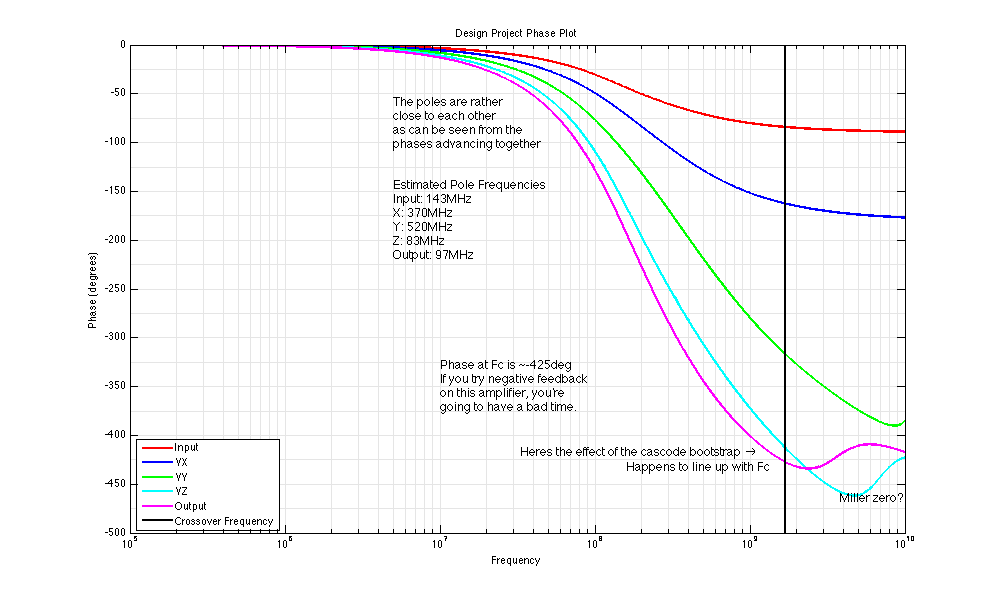
\includegraphics[width=1.1\textwidth]{phase.png}
\par}

\pagebreak

%%%%%%%%%%%%%%%%%%%%%%%%%%%%%%%%%%%%%%%%%%%%%%%%%%%%%%%%%%%%%%%%%%%%%%%%%%%%%%%%
% Transient Response - Page 8

% Show a transient simulation plot of the output for a 1 MHz, 1 µA sinusoidal
% input current. Make sure that there is no distortion.

\section{Simulated Transient Response}
\begin{figure}[h]
\centering
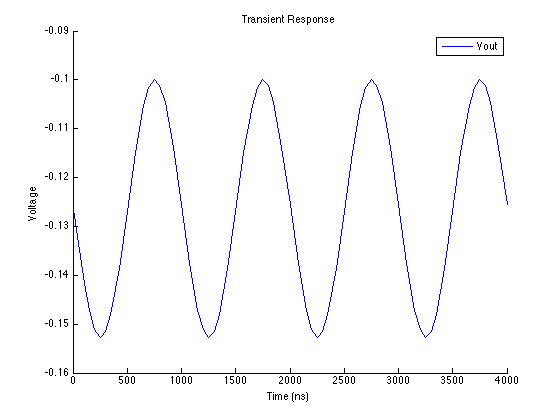
\includegraphics[scale=.75]{transient_response.png}
\end{figure}

\pagebreak


%%%%%%%%%%%%%%%%%%%%%%%%%%%%%%%%%%%%%%%%%%%%%%%%%%%%%%%%%%%%%%%%%%%%%%%%%%%%%%%%
% Comments and Conclusions - Page 9

% Comments and conclusion. Here, you can convey issues you may have had, or
% things you have learned/not learned in this project.

\section{Comments and Conclusion}


\begin{itemize}
\item Resistors contribute to a large part of the overall gain. From 
manufacturability perspective, passive components are not friendly and 
also occupy more area on the chip.
\item The output source follower stage is very sensitive to biasing due 
to back gate effect. Small variations on Vz can drive the output to fall 
out of desired common mode voltage or drive MN10 into cutoff region and 
lose all the gain from previous stages.
\item Any variations in supply voltage causes variation in Vov of MN7 
directly (as the device is biased through R3 \& R4) causing Vz to vary 
and thereby impacting the biasing of MN10 and gain.
\item Common source stage with diode connected load attributes to miller 
cap loading effect on cascade stage. This is limiting the gain of common 
source stage to smaller values.
\item Since the output is single ended, it is susceptible to noise. 
Differential configuration will be better.
\end{itemize}

\pagebreak

%%%%%%%%%%%%%%%%%%%%%%%%%%%%%%%%%%%%%%%%%%%%%%%%%%%%%%%%%%%%%%%%%%%%%%%%%%%%%%%%
% Spice Netlist - Appendix I

% Final SPICE netlist and .op output. Include only the MOSFET and node voltage
% listing from the .op output.

\section{Appendix I}
\begin{lstlisting}
* Design Problem, ee114/214A-2015
* Team Member 1 Name: Usha Kankanala
* Team Member 2 Name: Samuel Lenius
* Please fill in the specification achieved by your circuit
* before you submit the netlist
*************************************************************
* sunetids of team members:
*   ukankana@stanford.edu:  06091239
*   lenius@stanford.edu:    06091240
* The specification that this script achieves are:
* Power         1.06mW    <= 2.00 mW      Meets Spec
* Gain          34.6kOhm  >=  30.0 kOhm   Meets Spec
* BandWidth     93.0MHz   >= 90.0 MHz     Meets Spec
* FOM           3043      >= 1350         Meets Spec
*************************************************************

* Including the model file
.include /usr/class/ee114/hspice/ee114_hspice.sp


* Defining Top level circuit parameters
.param p_Cin = 220f
.param p_CL  = 250f
.param p_RL  = 20k

* Defining the supply voltages
vdd     n_vdd   0       2.5
vss     n_vss   0       -2.5

*Defining the input current source
** For ac simulation uncomment the following 2 lines**
Iin     n_iin   0       ac      100n
*Iin     n_iin   0       ac      1

** For transient simulation uncomment the following 2 lines**
*Iin    n_iin    0    sin(0 0.5u 1e6)

* Defining Input capacitance
Cin    n_iin    0    'p_Cin'

* Defining the load
RL      n_vout  0       'p_RL'
CL      n_vout  0       'p_CL'

*** Your Trans-impedance Amplifier here ***
***     d       g       s       b       n/pmos114       w       l

*** Vx/Iin = V(n_x) / Iin, use "n_x" as the node label for Vx ***
MN1     n_iin   n_bias_n  n_vss   n_vss nmos114 w=3.0u l=2.0u
MN2     n_x     0         n_iin  n_vss  nmos114 w=28.0u l=1.0u
MP3     n_x     n_bias_p  n_vdd  n_vdd  pmos114 w=6.0u l=2.0u
R1      n_vdd   n_x       19200
R2      n_x     0         20800

*** Vy/Vx = V(n_y) / V(n_x), use "n_y" as the node label for Vy ***
MP4     n_w     n_x       n_vdd  n_vdd  pmos114 w=6.0u l=1.0u
MP5     n_y     0         n_w    n_vdd  pmos114 w=6.0u l=1.0u
MN6     n_y     n_bias_n  n_vss  n_vss  nmos114 w=3.0u l=2.0u
R3      n_y     0         168100
R4      n_y     n_vss     34400

*** Vz/Vy = V(n_z) / V(n_y), use "n_z" as the node label for Vz ***
MN7     n_z     n_y       n_vss  n_vss  nmos114 w=2.0u l=1.0u
MP8     n_z     n_z       n_vdd  n_vdd  pmos114 w=2.0u l=1.0u

*** Vout/Vz = V(n_vout) / V(n_z), use "n_vout" as the node label for Vout ***
MN9     n_vout  n_bias_n  n_vss  n_vss  nmos114 w=5.0u l=2.0u
MN10    n_vdd   n_z       n_vout n_vss  nmos114 w=28.0u l=1.0u

*** Your Bias Circuitry goes here ***
MP100   n_bias_n n_bias_p n_vdd n_vdd  pmos114 w=4u  l=2u
MP200   n_bias_p n_bias_p n_vdd n_vdd  pmos114 w=4u  l=2u
MN300   n_bias_n n_bias_n n_vss n_vss  nmos114 w=2u  l=2u
MN400   n_bias_p n_bias_n n_biasr2   n_vss  nmos114 w=4u l=2u
R200    n_biasr2 n_vss  16.7k
MP800   n_biasn9 n_bias_n n_vdd n_vdd pmos114 w=2u  l=9u
MN700   n_biasn9 n_bias_n n_vss n_vss nmos114 w=5u  l=2u
MN900   n_bias_p n_biasn9 n_vss n_vss nmos114 w=4u  l=2u

*** defining the analysis ***
.op
.option post brief nomod

** For ac simulation uncomment the following line**
.ac dec 1k 100 1g

.measure ac gainmax_vout max vdb(n_vout)
.measure ac f3db_vout when vdb(n_vout)='gainmax_vout-3'

.measure ac gainmax_vx max vdb(n_x)
.measure ac f3db_vx when vdb(n_x)='gainmax_vx-3'

.measure ac gainmax_vy max vdb(n_y)
.measure ac f3db_vy when vdb(n_y)='gainmax_vy-3'

.measure ac gainmax_vz max vdb(n_z)
.measure ac f3db_vz when vdb(n_z)='gainmax_vz-3'

** For transient simulation uncomment the following line **
*.tran 0.01u 4u

.end
\end{lstlisting}
%\lstinputlisting[caption=Scheduler, style=customc]{}

\end{document}
